\documentclass[12pt]{article}
\usepackage{amsmath}
\usepackage{array}
% \usepackage{gensymb}
\usepackage{geometry}
\usepackage{graphicx}
\usepackage{pgfplots}
\usepackage{siunitx}
\usepackage{wrapfig}

\title{Homework \#11}
\author{Donald Aingworth IV}
\date{November 6, 2024}

\pgfplotsset{width=8cm,compat=1.9}
\usepgfplotslibrary{external}
% \tikzexternalize

\begin{document}

\DeclareSIUnit{\mile}{mi}
\DeclareSIUnit{\gal}{gal}
\DeclareSIUnit{\foot}{ft}
\DeclareSIUnit{\h}{h}

\maketitle

\pagebreak
\section*{Problem 1}
A neutron at rest decays into a proton, an electron, and a neutrino. If the proton's momentum is $3.00\times10^{-24}$ kg m/s in the direction 37\unit{\degree} N of E and the electron's momentum is $4.00\times10^{-24}$ kg m/s in the direction 53\unit{\degree} S of W, what is the momentum of the neutrino?

\subsection*{Solution}


\pagebreak
\section*{Problem 2}
\begin{wrapfigure}{r}{0.35\textwidth}
    \vspace{-30pt}
    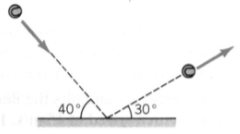
\includegraphics[width=0.35\textwidth]{graph_2.png} 
    % \label{fig:wrapfig}
\end{wrapfigure}
A 60.0-g tennis ball strikes the ground at 25.0 m/s at 40\unit{\degree} to the horizontal. It bounces off at 20.0 m/s at 30\unit{\degree} to the horizontal. (a) Find the impulse exerted on the ball. (b) If the collision lasted 5.00 ms, find the average force exerted on the ball by the court.

\subsection*{Solution}


\pagebreak
\section*{Problem 3}


\subsection*{Solution}


\pagebreak
\section*{Problem 4}


\subsection*{Solution}


\pagebreak
\section*{Problem 5}


\subsection*{Solution}


\pagebreak
\section*{Problem 6}


\subsection*{Solution}


\pagebreak
\section*{Problem 7}


\subsection*{Solution}


\pagebreak
\section*{Problem 8}


\subsection*{Solution}

\end{document}